\chapter{Contas Públicas Estadual}
\section{Receitas e Despesa do
Estado}
As contas do Estado até agosto de 2020 está em melhor situação quando
comparado ao mesmo período de 2019, até agosto de 2019 o resultado
primário, diferença entre receita e despesa primário não financeira, foi
de cerda de R\$622 milhões, em 2020 o resultado foi de pouco mais de
R\$1 bilhão de reais. O resultado primário representa o esforço fiscal
do governo para diminuição do estoque da dívida, basicamente se o
governo apresenta um resultado primário negativo, isto é, um déficit
primário, ele necessita financiar seu gastos elevando a dívida, o
inverso, quando se apresenta superávit primário há um esforço no sentido
de diminuir dívida. A Figura xx apresenta variação da receita e despesa
primária do Tocantins até o bimestre em relação ao mesmo período do ano
passado.

Em todos os bimestre de 2020, a despesa primária cresceu a uma taxa
maior que a receita primária, exceto para o quarto bimestre, o que não
se traduz em elevação da dívida, mas se a tendência persistir, i.e, uma
taxa de crescimento da despesa acima da receita, irá gerar desequilíbrio
e elevação da dívida. Observa-se que embora a despesa cresca à uma taixa
mais elevada, ela vem caindo desde o primeiro bimestre, onde cresceu
mais de 30\% quando comparado ao primeiro bimestre de 2019. No quarto
bimestre de 2020 a receita superou a despesa.

O crescimento da despesas primária nos primeiros bimestre de 2020, se
deve em boa parte a um crescimento das despesas com pessoal e encargos
sociais, essas se referem a gastos com pessoal ativo, inativo,
pensionistas entre outros. No primeiro bimestre de 2020, essa conta
cresceu 37,89\% em relação ao mesmo período do ano passado. No acumulado
até agosto o crescimento foi de apenas 0,76\%.

\begin{figure}[h]
\caption{Variação da Receita e Despesa Primária em relação ao mesmo período ano passado}
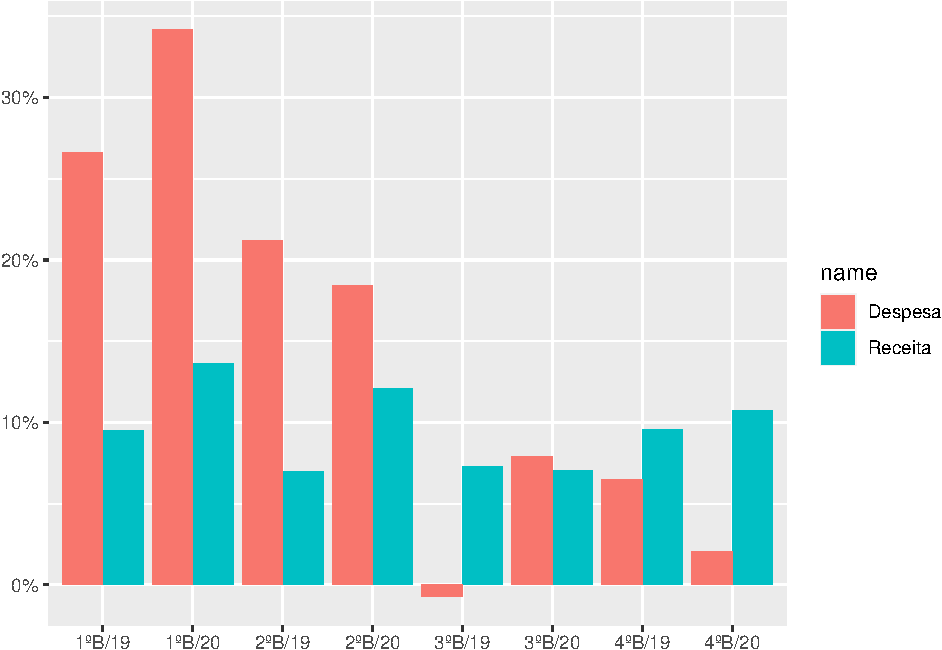
\includegraphics[width=\linewidth]{fig/unnamed-chunk-4-1.pdf}
\end{figure}

\begin{figure}[h]
\caption{Variação da Despesa por Função em relação do mesmo perído do anopassado}
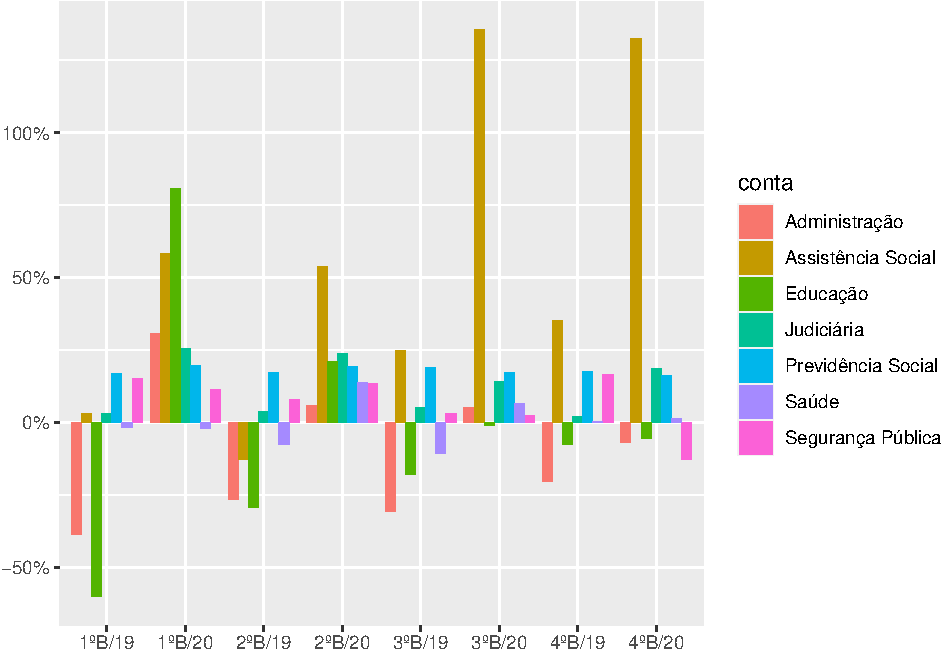
\includegraphics[width=\linewidth]{fig/unnamed-chunk-6-1.pdf}
\end{figure}
A Figura xx mostra as despesas por função, despesas com judiciário e
previdência social tiveram um crescimento real no acumulado até agosto
quando comparado ao mesmo período de 2019, os gastos com judiciário
cresceram cerda de 18\% e com previdência social aproximadamente 16\%.
Os gastos com assistência social cresceram substancialmente, mas tiveram
pouco impacto na despesa, até o quarto bimestre o governo gastou R\$49
milhões.

Administração, Educação e Segurança Pública encolheram seus gastos no
quarto bimestre de 2020, em 2019 educação e administração já
apresentavam encolhimento em relação à 2018.

As despesas com pessoal em relação a receita corrente líquida, Figura
XX, descreve o quanto da receita foi para despesas com pessoal no
acumulado do ano. A Lei de Responsabilidade Fiscal impõe limites para
gastos com pessoal, para o executivo estadual o limite máximo é de 49\%.
Caso o executivo ultrapasse 95\% do limite prudencia
(\(95\%\cdot46.55\%=42.22\%\)), fica vedado criação de cargos,
reajustes, entre outros que caracterizem aumento da despesa. Até agosto
de 2019, a relação despesa/receita ficou em 47,67\%, abaixo do limite
máximo, mas acima do limite prudencial. Para esse ano, o estado não
ultrapassou o limite prudêncial, por uma pequena margem. Um recuperação
na receita ao longo do último quatros meses sem alterar as despesas com
pessoal pode deixar o estado abaixo do limite prudencial.

\begin{figure}[h]
\caption{Despesa Total com pessoal em Relação a RCL}
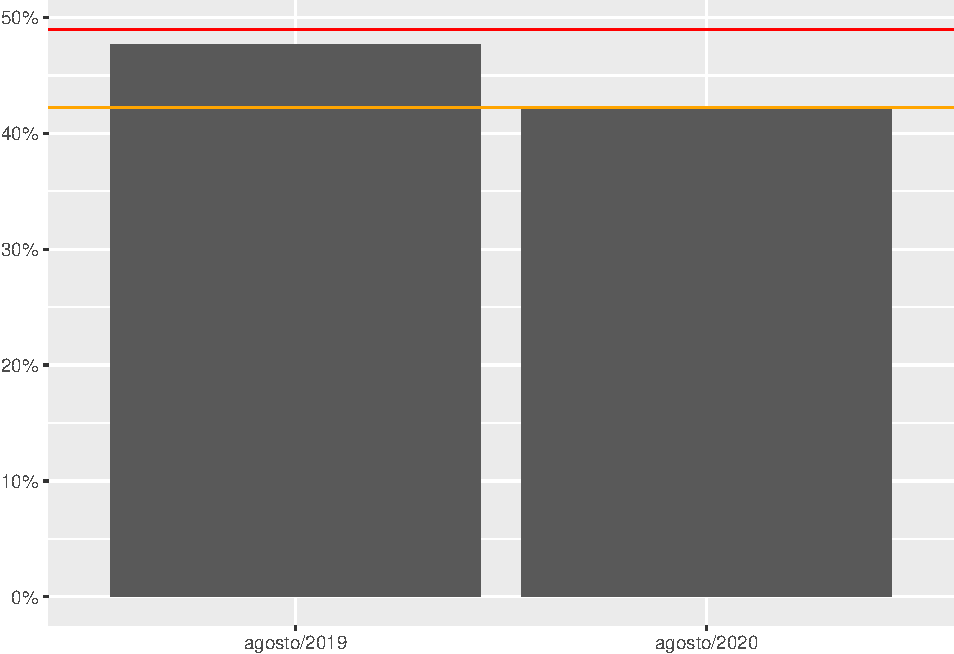
\includegraphics[width=\linewidth]{fig/unnamed-chunk-8-1.pdf}
\end{figure}

\section{Capacidade de Pagamento do
Estado}
O cálculo da capacidade de pagamento (CAPAG) traz informações a cerca da
situação fiscal do Estados e Munícipois. A nota é utlizada para Estados
contrair empréstimos com garantia do Governo Federal. A nota atribuida a
cada Estado ou Município é derivada de três indicadores: endividamento,
poupança corrente e liquidez. Em 2020 apenas o Espírito Santo obteve
nota A. O Tocantins ficou com nota C por três anos seguidos. Notas A e B
permite que o Estado receba garantia da União para pedi novos
empréstimos.

Dos Estados da região, os que apresentaram pior nota foi Roraima e
Tocantins. Rondônia aparece como o Estado com melhor evolução, melhorou
sua nota de B para A entre 2019-2020, a queda no endividamento de
65,41\% para 57,6\% e a redução na relação obrigações
financeiras/disponibilidade de caixa, diminuindo sua liquidez para
19,1\% garantiu nota A em todos as categorias do CAPAG.

O Tocantins apesar se manter a mesma nota, teve pioras em todos os
indicadores: endividamento, poupança corrente e liquidez. O seu
endividamento que é a dívida consolidada bruta em relação a receita
corrente líquida aumentou de 46,35\% para 67,6\%, a poupança corrente
que corresponde a relação despesas correntes e receita correntes
ajustadas também apresentou uma pequena piora, de 94,56\% para 95,9\%.
Quanto menor o índice de poupança corrente melhor, pois melhor será a
capacidade da receita corrente de financiar investimentos. O último
indicador é o de liquidez, para obter nota A, o Estado ou Município deve
ter um índice menor que 100\%, o que significa que sua disponibilidade
em caixa é maior que suas obrigações financeiras. O Tocantins tem um
índice de 577,5\%, em 2019 era 539,40\%.

De todos os indicadores do Estado, endividamento e poupança corrente
estão em melhor situação, pois estão mais próximo do limite para receber
uma melhor nota. Para conseguir uma nota A no índice de endividamento o
Estado deve conservá-lo abaixo de 60\%, atualmente está com 67,6\%. No
índice de poupança corrente, para garantir uma nota B o índice deve
maior ou igual a 90\% e menor que 95\%. Para uma nota A, basta que seja
menor que 90\%, atualmente está em 95,9\%, bem próximo de 95\%.

O índice de liquidez é uma situação mais delicada, ele tem maior peso na
nota final, para que um Estado ou Município obtenha nota A no CAPAG.
Para ter uma nota B é necessário obter A no índice de liquidez e nota
acima de C na poupança, independente da nota do endividamento. Logo
nota-se sua importância, pois se o Estado busca melhorar sua nota tem
que pelo menos ter A de liquidez. O Tocantins tem 577,5\% de liquidez,
valor muito acima de 100\%. O esforço logo deve ser maior nesse índice
caso queira obter uma melhora, o caminho é melhorar a relação obrigações
financeiras e disponibilidades de caixa bruta, ou diminuindo as
obrigações em relação a disponibilidade, ou o inverso, aumentando a
disponibilidade, isto é, ativos de alta liquidez, e diminuir as
obrigações.

\begin{tabu} to \linewidth {>{\raggedright}X>{\raggedleft}X>{\raggedleft}X>{\raggedleft}X}
\toprule
UF & 2018 & 2019 & 2020\\
\midrule
AC & B & B & B\\
AL & B & B & B\\
AM & B & B & B\\
AP & B & C & Suspensa\\
BA & C & C & C\\
\addlinespace
CE & B & B & B\\
DF & C & C & C\\
ES & A & A & A\\
GO & C & C & C\\
MA & C & C & C\\
\addlinespace
MG & n.d. & D & D\\
MS & C & C & C\\
MT & C & C & C\\
PA & B & B & B\\
PB & B & B & B\\
\addlinespace
PE & C & C & C\\
PI & C & B & C\\
PR & B & B & B\\
RJ & D & D & D\\
RN & C & C & C\\
\addlinespace
RO & B & B & A\\
RR & C & C & C\\
RS & D & D & D\\
SC & C & C & C\\
SE & C & C & C\\
\addlinespace
SP & B & B & B\\
TO & C & C & C\\
\bottomrule
\multicolumn{4}{l}{\rule{0pt}{1em}\textit{Note: }}\\
\multicolumn{4}{l}{\rule{0pt}{1em}Boletim de Finanças dos Entes Subnacionais 2020}\\
\end{tabu}

\begin{tabu} to \linewidth {>{\raggedright}X>{\centering}X>{\centering}X>{\centering}X>{\centering}X>{\centering}X>{\centering}X}
\toprule
\multicolumn{1}{c}{ } & \multicolumn{2}{c}{Endividamento} & \multicolumn{2}{c}{\makecell[c]{Poupança\\Corrente}} & \multicolumn{2}{c}{Liquidez} \\
\cmidrule(l{3pt}r{3pt}){2-3} \cmidrule(l{3pt}r{3pt}){4-5} \cmidrule(l{3pt}r{3pt}){6-7}
UF & 2019 & 2020 & 2019 & 2020 & 2019 & 2020\\
\midrule
AC & B & B & B & B & A & A\\
AM & A & A & B & B & A & A\\
AP & B & B & A & A & A & -\\
PA & A & A & B & B & A & A\\
RO & B & A & A & A & C & A\\
\addlinespace
RR & A & A & A & A & C & C\\
TO & A & B & B & C & C & C\\
\bottomrule
\end{tabu}
